\section{Introduction}
\label{s:Literature-Introduction}
Documentation is a crucial aspect of the development of software. It is so
important that every developer building a GraphQL API should be aware of it an
keeping their Schemas documented to enable and facilitate consumers to
understand how to use the API \citep{derksDocumentingGraphQLAPIs2021}. A very a
good way to document such APIs is not to be locked in with any vendor-specific
that generates documentation on the fly given a specific schema but building
static documentation that automatically updates on the fly when a change is made
to it (ibid). The following literature review will point the differences between
different APIs, analyse and critically evaluate the options developers have to
reach the same goal and why the software implementation of the tool used in the
project gives the producers better results, freedom and save them money. Security
implications are also another important aspect of the lifecycle and this paper
will dive into analysis and confrontation to understand this.


\section{GraphQL Security and Performances}
\label{s:GraphQLSecurity}
\citet{hartigInitialAnalysisFacebook2017} define GraphQL as a new form of
web-based connectivity interface that provides alternatives concept of
REST approaches. Due to its benefits over REST, the subject of this paper (GraphQL) has gained
popularity since its debut. GraphQL has grown in popularity and is being used by
many users. GraphQL is a novel technique of interacting using APIs. According to
\citet{ vogelExperiencesMigratingRESTful2018}, GraphQL is not a database
technology, as many people believe. Users may already be aware that most modern
applications save their data on a distant server in a database, and here is
where GraphQL comes in. Simply providing a means of accessing data required by
the application is all required by the API. REST APIs may also be built with
GraphQL \citep{vadlamaniCanGraphQLReplace2021}. It was created internally by
Facebook for various purposes before being made open-source and made available
to the public. Because of this, it has become one of the most used technology
stacks for building online services. GraphQL is a query language that specifies
how an application program can ask a distant server for the data it needs.
Consequently, the requested client query receives a response from the server app.
Client applications may inquire about what they need without relying on their
server-side counterparts for guidance. \citet{
hartigDefiningSchemasProperty2019}, in their research study, has focused on
repurposing schemas for graphs, which was initially intended as a language that clarifies
various kinds of things, which can be queried when attempting to access a
particular Web API. The perspective of data use GraphQL have a
schema to express the shape of the graphs (ibid). Many different viewpoints
have been put together by the same author in his paper to define GraphQL schemas
in terms of their quantitative definitions
\citep{hartigInitialAnalysisFacebook2017}. GraphQL is sometimes described as an
edge-labelled multi-graph with a dictionary of attributes, wherein every node is
connected with an object type. \citet{britoMigratingGraphQLPractical2019} have a
case study on migrating API customers to this new technology in this article.
First, they surveyed the grey literature to acquire a thorough knowledge of the
benefits and essential qualities of the technology that practitioners typically
connect with. Following that, \citet{britoMigratingGraphQLPractical2019}
demonstrate these benefits in reality by moving seven services to GraphQL rather
than typical REST-based APIs. As a crucial finding, the researchers demonstrated
that it could significantly minimize the volume of JSON records supplied by REST
APIs (ibid). In blog, \citet{kristopherUniqueBenefitsUsing2018}
outlined the benefits of utilising the graph. He points that since it is so
strong, it has been employed by some service providers who require a high level
of accessibility and indexing speed. For the most part, the practical
applications for GraphQL are those that need fast data flow and easy sorting and
representation by its most high-profile customers. An architectural model's
specific performance characteristics may be gleaned via studies on response time
and average transfer rates between requests, as noted by
\citet{seabraRESTGraphQLPerformance2019}. Two-thirds of the evaluated
applications found that moving to GraphQL led to a performance boost. After
constructing REST and GraphQL API endpoints and testing them in an open-source
playground, Seabra et al. performed a PoC not by transitioning to
GraphQL but rather by establishing prototype API endpoints for both testings the
response time for data extraction across three iterations. In the first
iteration there was little or no change when we investigated a single API
endpoint for GraphQL and REST with the 1000 data records quantity
\citep{seabraRESTGraphQLPerformance2019}. In the second iteration there was a
35\% faster response time utilizing GraphQL, despite a tenfold increase in data
volume than Iteration 1 and Iteration 2 were conducted with 10000 data records
(ibid). In the third iteration, whenever Seabra et al. raise the quantity of
data 100 times the initial quantity and run using one hundred thousand records, they
evaluate three endpoints rather than the needed one (ibid). The
researchers suggested a roughly 40\% reduction in reaction time needed in
the GraphQL experiment findings. According to Seabra et al. among software
development experts, the subject of which architectural model to adopt is
frequently asked: This topic of performance has been answered by examining the
performance of three different target apps, each of which was built utilizing
two different web services architectural models: REST and GraphQL. Every
architectural model's performance indicators may be deduced from the study of
reaction time and average transfer rates. Migration to GraphQL led to a dramatic
increase in the average demand per second and information transfer rates in
various evaluated apps. After the migration research, it was shown that
GraphQL-based services performed worse than their REST-based counterparts for
loads exceeding three thousands requests, varying 99 to 2160 KB/s. Both
REST and GraphQL services performed similarly for simple workloads, with values
ranging from 6 to 7 requests each second for work of one hundred requests between
GraphQL and REST services. Researchers at Salt Security's Salt Labs discovered
the flaws in the FinTech firm's mobile apps and SaaS platform while doing their
study. Problems stemmed from a lack of authorisation and nested queries being
prone to many mistakes. Salt Labs discovered that the researchers might submit
operations against any user's account or capture any customer's sensitive data
if proper authorisation checks were not implemented (Vadlamani et al., 2021). A
report from Salt Security shows that 62\% of firms have no or a minimal
API security policy \citep{vadlamaniCanGraphQLReplace2021}. A basic attack like
not verifying or cleaning the API queries may lead to trouble. According to
\citet{britoRESTVsGraphQL2020}, GraphQL is becoming increasingly popular as a
preferable API management platform in environments with high data volumes, where
response speed and the usage of fewer API endpoints are essential performance
indicators. Although REST is becoming an enterprise standard and API
administration utilising REST endpoints has evolved, GraphQL has a learning
curve. With enhanced tooling features over time, future uses of GraphQL will
rise manifold. This research spur other researchers to pursue the goal of flexibility and performance with minimal involvement.
Several GraphQL implementations allow Introspection by default, which means they
may be accessed without authentication \citep{eizingerAPIDesignDistributed2017}.
The fact that Introspection enables the requester to understand all of the
available schema and queries is troublesome. API owners may use Introspection to
inform users about the API's workings and potential pitfalls. Users prefer to
learn about a service via a distinct documentation channel like a Git Readme or
reading the manuals. The safest and most convenient option is deactivating
Introspection and the GraphiQL scheme (ibid). If disabling Introspection is not
supported natively by the implementation, or if users want to provide this
access to certain users or roles, therefore may create a filter in the service
that restricts access to the introspection system to those users who have been
allowed by the service's administrators. Even if Introspection is turned off, an
attacker might still brute force fields to estimate their values. As a bonus,
GraphQL comes with a built-in hinting function suggests a working query based on
whenever a requester's field title is close (but wrong) to an already-existing
field. Not all installations of GraphQL enable this functionality; therefore,
users should consider deactivating it if they want to reduce their exposure
\citep{kouraiSecureOffloadingLegacy2016}. A tool like Shapeshifter might be able
to help with this. Disabling Introspection is a sort of security via obscurity
since bad actors still may learn ways to construct harmful queries by
reverse-engineering the GraphQL API using several trials and errors (ibid). When
used with additional security measures such as volumetric quotas and operation
safe listing, it is not the most excellent protection method. It is possible to
examine all schema data using GraphQL Introspection. When Introspection is
enabled in production, it makes it easier for hostile actors to find graph
weaknesses, such as disclosing sensitive information. Using a schema registry to
record the graph and metadata is safer and more secure. SQL injection, OS
Command Injection (SSRF/CRLF), NoSQL injection, and DoS attacks may all be
prevented by disabling Introspection (Denial of Service) \citep{
eizingerAPIDesignDistributed2017}. Attacking the API's accessibility and
stability is a form of DoS, which can cause the API to be sluggish, unresponsive,
or inaccessible \citep{gozneliIdentificationEvaluationProcess2020}. There is a
fair chance the target has Introspection turned off, so take advantage of this.
GraphQL backends come pre-loaded with proposals for fields and functions.
GraphQL may offer fields equivalent to the original query if users try to query
the field but make a typo. Hackers can use the Field Suggestion functionality to
learn more about
GraphQL's schema, even though it is not vulnerable (ibid). An investigation on
timeouts in GraphQL was conducted by \citet{ witternEmpiricalStudyGraphQL2019}.
Adding timeouts is a straightforward approach to limit the number of resources a
single request may use. The problem is that timeouts do not always work since
they do not kick till a malicious query has used a large amount of computing
power. There is not a single timeout number that will work for all APIs and data
fetching mechanisms. If desired, queries and resolver functions can set timeouts
at the application level. Because the timeout has been reached, this technique
is typically more effective. Request timeouts cannot be implemented natively in
GraphQL due to technical limitations. The proliferation of APIs has resulted in
a rise in attempted assaults with automated apps executing harmful operations
via the Application Programming Interfaces \citep{
hartigInitialAnalysisFacebook2017}. As per research from wallarm.com, harmful
bots now account for up to 20\% of the internet. As a result, protecting
APIs is a vital component of application security. GraphQL and REST API
development lifecycle techniques are helpful in certain situations, and each has
its own set of perks and downsides. GraphQL is growing in popularity at a
breakneck pace, owing primarily to its ``no over and under-fetching'' capability
(ibid). It enables more effective client-side communication and is an
instrumental and powerful technology, particularly as the software sector
transitions to an agile framework. GraphQL is a mechanism for accomplishing
specific query-oriented goals; nevertheless, it is not a panacea for all
API-related difficulties and is not a substitute for REST. When frontend
development teams consume REST APIs, they must wait for the backend team to
complete creating the APIs necessary for the client application to collect and
send data. The complete development process is entirely dependent on the
creation and delivery of the REST API. The GraphQL lifecycle method is
significantly different and more efficient, allowing frontend and backend
programmers to operate concurrently without impeding the whole development
process. GraphQL's essential quality is that it is less verbose than REST APIs.
GraphQL prioritises speed above everything else, whereas REST prioritises
service dependability. It does not matter whether the REST API provides only a
simple partial because it is still sending more data than is necessary
\citep{vadlamaniCanGraphQLReplace2021}. The API can add new fields to the
GraphQL query, but clients do not get them until they explicitly request them.
REST is slower since users cannot select which fields to query; therefore, the
request will be as minimal as possible, making it quicker with GraphQL. Since
GraphQL transfers fewer bits over the wire, the applications will run quicker
than when using REST. Furthermore, developers may query several entities at
once using GraphQL \citep{lawiEvaluatingGraphQLREST2021}. Unpredictable APIs are
of no utility. As a result, every program that uses an API must be aware of what
it may call and how it can anticipate and act on the API's output appropriately.
In other words, an API's explanation of what may be accessed is critical.
GraphQL introspection and REST API schema frameworks such as Swagger allow
developers to explore programmatically the information they gain from the API
documentation. Concerning security, REST appears to have the upper hand when
comparing GraphQL to REST. API security may be enforced in several ways using
REST \citep{vadlamaniCanGraphQLReplace2021}. For example, one may secure REST
APIs by supporting several API authentication methods, such as the HTTP
authentication mechanism. JSON Web Tokens, HTTP headers, or OAuth 2.0 protocols
can all transmit private information, such as passwords and credit card numbers.
In addition to REST, GraphQL has certain security features; however, they are
not as developed as REST's GraphQL \citep{lawiEvaluatingGraphQLREST2021}. For
example, it helps integrate data validation, but users must figure out how to
implement permission and authentication procedures on top. In his research,
\citet{vadlamaniCanGraphQLReplace2021} investigated whether REST can replace
GraphQL. In API development, REST has long been the go-to architectural approach.
In 2015, Facebook announced GraphQL, which has since challenged GraphQL's
popularity. GitHub, Airbnb, Shopify, Twitter, and many other internet platforms
have already implemented it (ibid). Many questions remain unanswered about the
efficiency and viability of GraphQL's application, even if it offers a
significant improvement over REST. This article evaluates the quantity and
quality viability of adopting GraphQL over REST for API design. When it comes to
API response speeds, GitHub has built a unique API client that can be used to
measure the change between REST and GraphQL. After that, a GitHub workers poll
was conducted to understand better what REST and GraphQL mean in software
engineers' experience with APIs. Both API paradigms have advantages and
disadvantages, and none can substitute the other. There is a clear preference in
the GraphQL versus REST argument for REST APIs. A State of API 2020 report found
that 82\% of API customers and practitioners utilise REST-based OpenAPI
authentication, whereas just 18\% use GraphQL (ibid). There has also been a
steady rise in GraphQL's popularity. JavaScript use has increased from 5\%
in 2016 to 38\% in 2019, as per the State of JavaScript 2019 Report
(ibid). Today, most browsers support the HTTP cache so that resources are not
re-fetched. It can also be used to tell if two factors are identical in any
other way. In GraphQL, users cannot use the same URL for all requests to receive
a globally unique id for an item. For this, one will need to configure the
GraphQL cache.

\section{GraphQL vs REST}
\label{s:GraphQLvsRest}

Before diving in, context needs to be added on why the projects build solutions
for GraphQL instead of REST. REST has become the common choice to build and
design APIs in the past years \citep{britoRESTVsGraphQL2020}, but as the
developers needed more flexibility on evolution, a sharp decouple between the
backend and frontend and a gateway to access all the data they needed through a
single point of access. GraphQL came to the rescue of such developers wanting a
better way to build API. While REST usually have multiple endpoints to fetch
different type of data, GraphQL unifies everything through a single query to the
server with a simple JSON return with the data requested by the consumer. One of
the biggest problems of REST is overfetching. Designing an API that returns
exactly what the consumer wants in REST requests is impossible
\citep{seabraRESTGraphQLPerformance2019}. GraphQL solved the overfetching
problem as the user can write a specific query with the data needed. As
previously mentioned, GraphQL - differently from REST - is decoupled from the
backend. That means the front end can change its UI without changing the back
end for adjustments. Not only for the same reason, but the backend also has
instrumental analytics on the data requested by the consumer since everything
will be requested through a specific query. That leads to supporting graceful
deprecation of specific fields that are not mainly used. That is alluring, but
how does a consumer know which query to write to gather his data? This is when
Introspection comes in handy, but it has some critical drawbacks and security
implications that makes it unusable in production. Contrary to all the
advantages previously explained, the team at
\citet{stablekernelAdvantagesDisadvantagesGraphQL2021} also emphasised many
disadvantages. One of that is that every query always returns a state of 200
even if the query was not successful. It is very accurate and changes the way of
monitoring and measuring errors from how everyone is used with REST. GraphQL is
also very bad at handling caching which is also very complex to implement and
manage, but one thing that has not been mentioned from
\citet{stablekernelAdvantagesDisadvantagesGraphQL2021} is that it is also fairly
simple to wrap the whole API in a Content Delivery Network (CDN) that would be
the first point of contact between the server and the consumer. There are many
very viable techniques that would make this solution not only a patch to what
GraphQL does badly, but also to generally improve the API. A CDN could fully
cache any document and not only small pieces of it, making it very fast, secure,
scalable and on edge, which is always a great addition to services such as an
API.

\subsection{Introspection}
\label{s:Literature-Introspection}

Introspection is a GraphQL feature that, if enabled, grant access to a query
that returns any possible query and updates as the schema evolves overtime. A
bad actor could easily access sensitive information, types, and operations
supported with such a tool.

\begin{figure}[ht]
	\centering
	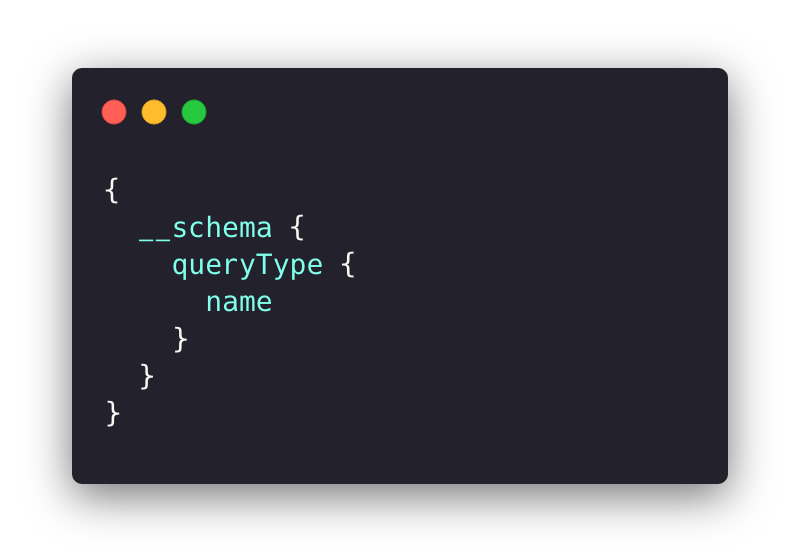
\includegraphics[width=0.5\textwidth]{figures/code/introspection.png}
	\caption{Introspection Query}
	\label{f:Introspection-Query}
\end{figure}

Introspection enables users to query a GraphQL API and discover its schema
structure, giving bad actors a chance to find potentially malicious operations
\citep{khalilWhyYouShould2021} quickly and disrupt the availability of the API.
However, it is also a requirement for tools such as \textit{GraphiQL} and
\textit{Playground}. This is a severe dilemma for producers who want to keep
their APIs as secure as possible, away from indiscreet eyes, and closed to
potential threats but still have documentation tooling. If the attackers have
access to the whole schema through introspection, it will be effortless to find
and exploit API calls meant for internal use and debugging purposes
\citep{rizwanGraphQLCommonVulnerabilities2021}. Through the same technique, the
attackers could also get access to mutations and API calls intended to add, edit
or delete specific data on the database, making it a real threat. Many other
security issues are linked to the activation of the introspection and
misconfiguration; some are information disclosure, insecure direct object
references, and inexistent Access Control List (ACL) \citep{
yeswehackHowExploitGraphQL2021}.

\subsection{N+1 Problem}
\label{s:N1-Problem}
By design, GraphQL has a fetching inefficiency known as \textit{N+1 Problem}
where the number of queries executed against the database (or other upstream
services) can be as large as the number of nodes in the resulting graph \citep{
graphqlbypopSuppressingProblemGraphQL2020}.
\begin{figure}[H]
  \centering
  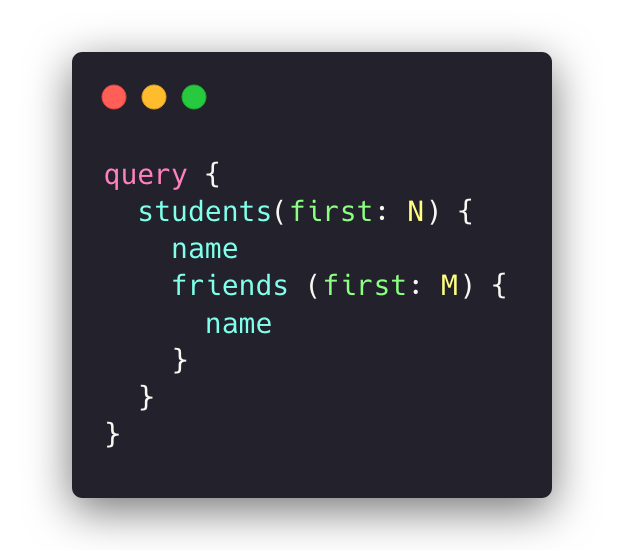
\includegraphics[width=0.5\textwidth]{figures/code/n+1}
  \caption{GraphQL N+1 Problem}
  \label{f:GraphQL-N1-Problem}
\end{figure}
In the example above, the query against the schema would make a single call to
the database to retrieve the first N students, and then for each of these Ns
students it would make a separate query to the same database to fetch M friends
details (N calls), hence N+1. Having introspection disabled is the right choice
looking at a security perspective, and this project will help solve the downside
of not having tools to help document the API and more.

\section{Exploring GraphQL API}
\label{s:Literature-ExploringGraphQLAPI}
There are different tools which lock-in both producers and consumers that aims
to explore a specific GraphQL API. The problem with those tools is that the
producer does not ever have the freedom and the flexibility to have a static
documentation running on a machine. Not only, most of the time the GraphQL
server needs to be communicating with the service, with introspection enabled.
Apollo Studio is a great tool to explore GraphQL APIs with just registering a
schema but it is a paid tool and does not come cheap. Also, in order to use most
of the tooling offered from Apollo, the server must be built with Apollo server
and this hugely lock the company or developer of the project to a single vendor
with huge implications in terms of flexibility and ownership of the whole
ecosystem that will be built around it. In practical terms, if a producer do
want to create a GraphQL API in Elixir using Absinthe \citep{
hexdocsOverviewAbsintheV12022}, it will be impossible for the developer to
utilise any of the Apollo tooling.

\section{Framework Agnostic}
\label{s:Framework Agnostic}
As previously mentioned, the end goal is to build a framework agnostic tool,
meaning that using a single GraphQL schema as a source of truth, the tool will
generate a well structured set of markdown files to document the API and utilise
those files in any way the developer wants. This would boost productivity and
flexibility as the developers can utilise the deep knowledge they already have
on a framework of their choice, with the language of their choice \citep{
stefanReasonsWhyWent2018}.

\section{GraphQL Schema}
\label{s:Literature-GraphQLSchema}
A GraphQL schema is a set of structured rules that express requirements for an
application. It might be easy with a simple UI but it can easily become
difficult as the interface of the application grows and evolves. It is to keep
in mind that most of the benefits that GraphQL brings to the table are
attributed to the schema itself as it enabled most of the features that GraphQL
provides such as code generation, parsing, validation and type checking. For
this exact reason, many developers couple GraphQL with a strong typed language
such as TypeScript to have an ecosystem of tools at their disposal that can help
them catch errors at runtime through the IDE or editor itself, rather than at
compile time. The GraphQL schema is also a graph because not only is a
representation of data graph but also a definition of relationships between
entities \citep{karthicDesigningGraphQLSchemas2020}. That are few in-built
types that are covered in GraphQL which are Object, Scalar, Query and Mutation.
The Scalar types that GraphQL supports are Int, Float, String, Boolean and ID.
All these specs will be covered and supported in the project as it is very
important to support all the types that are built-in GraphQL or the
documentation would fail to be procued as the schema could have types not
supported. An example of object type below.

\begin{figure}[H]
  \centering
  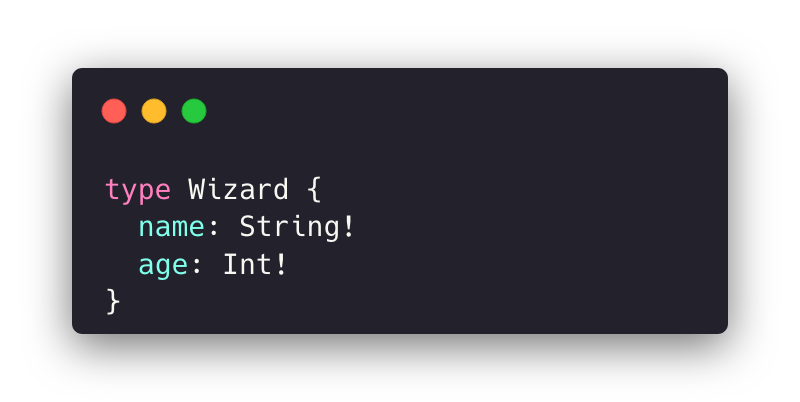
\includegraphics[width=0.5\textwidth]{figures/code/wizard}
  \caption{Object Type}
  \label{f:Wizard-Object}
\end{figure}

In this object type there are also two scalar type as field which represent
the decoration of their entities. In this case both fields are both non-nullable
fields, which means that the field cannot be null and is mandatory. Meaning that
if a consumer performs a query on a non-nullable field, he will never be able
to receive a response like the one below.

\begin{figure}[H]
  \centering
  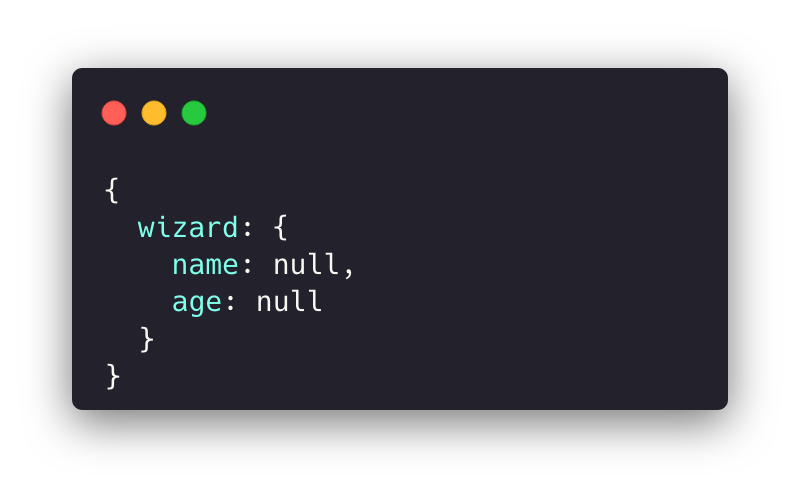
\includegraphics[width=0.5\textwidth]{figures/code/wizardresult}
  \caption{Wizard Query Result}
  \label{f:Wizard-Query-Result}
\end{figure}


\section{MD and MDX}
\label{s:MDandMDX}
As \citet{gruber38MarkdownSyntax2020} explains in his article, Markdown is
intended to be simple to read and simple to write. It is important to have a an
output text that is easy to read so that the end consumer does not have to know
anything related to coding to make things as simple as possible. In this case,
though, we also want to embed and integrate components in our markdown files,
hence the use of the MDX. It is fair to say that MDX is a superset of MD that
blends both markdown and JSX syntax to build an hybrid to power the most modern
frameworks such as React, Vue and Angular, but still leave the choice to the
developers building the project.

\section{Conclusion}
\label{s:Literature-Conclusion}
Developers are not only interested in building an API but also in continously
document it and provide a way for their consumers to have a better understanding
of the API. Even though GraphQL could have some downsides, the advantages of
using it are just far too greater to ignore. A tool to create documentation
while keeping the schema and the structure of the API secure and keeping
everything framework agnostic is something that this project will try to achieve.
After some research it is easy to say that it will be unique and could be
interesting to see how it could expand after making it open-source.
